
%----------------------------------------------------------------------------------------
%	CHAPTER 
%----------------------------------------------------------------------------------------
\chapterimage{chapter_head_2.pdf} % Chapter heading image

\chapter{Treinando o \bodyisolation}
\label{chap:trainingbodyisolation}

Como já foi mencionado na Seção \ref{sec:BodyIsolation} os movimentos 
com isolamento corporal (movimentos policêntricos) são muito comuns
nas danças de raiz africana, pois músicas \hyperref[subsec:polirritmia]{\textbf{polirrítmicas}}
em geral provocam danças policêntricas. 
Consequentemente, o samba de gafieira,
que ostenta uma profunda conexão com as danças africanas,
também tem o isolamento corporal como caraterística. Assim,
em muitos momentos de nossa dança perceberemos que será necessário 
desassociar os movimentos da parte superior do corpo (tórax e braços)
dos movimentos da parte inferior (pernas),
gerando desta forma um conjunto de torções e posturas que são caraterísticos do samba de gafieira. 
%%%%%%%%%%%%%%%%%%%%%%%%%%%%%%%%%%%%%%%%%%%%%%%%%%%%%%%%%%%%%%%%%%%%%%%%%%%%%%%%
%%%%%%%%%%%%%%%%%%%%%%%%%%%%%%%%%%%%%%%%%%%%%%%%%%%%%%%%%%%%%%%%%%%%%%%%%%%%%%%%
\section{Treinamentos de desassociação corporal}

A continuação serão listados um conjunto de exercícios que nos ajudarão a melhorar 
o controle corporal e a desassociar algumas partes de nosso corpo.

\begin{example}[Treinando com movimentos policêntricos - ombros e pés:]
Neste exercício buscaremos desassociar os movimentos dos ombros
dos movimentos dos pés.
Para que a desconexão dos movimentos seja treinada a nível cognitivo-motor,
estabeleceremos a condição de que os ombros e pés se movimentem de forma simultânea,
porém seguindo ritmos diferentes.
\begin{itemize}
\item Os ombros serão movimentados seguindo um ritmo ``tchic tchic tum'', 
\meter{2}{4}\leftrepeat~\Vier\Acht\Acht~\rightrepeat, enquanto que 
\item os pés se movimentarão seguindo um ritmo ``tum tum'', 
\meter{2}{4}\leftrepeat~\Vier\Vier~\rightrepeat.
\end{itemize}
Como fonte de informação musical podemos usar qualquer melodia de samba de nossa preferencia,
ex: ``Rio antigo'' interpretado por Alcione,
ou alguma melodia simples gerada sinteticamente, 
como a mostrada na Figura \ref{fig:bodycontrol1-poliritmia-1}.
Nesta figura temos dois instrumentos musicais que são executados ao mesmo tempo,
o pandeiro corresponde ao movimento de ombros e as claves ao dos pés.
Qualquer que seja a música escolhida, nosso objetivo será manter-nos
caminhado com pisadas em tempo enquanto marcamos um ritmo ``tchic tchic tum'' com os ombros.
\end{example}
\begin{figure}[!h]
  \centering
    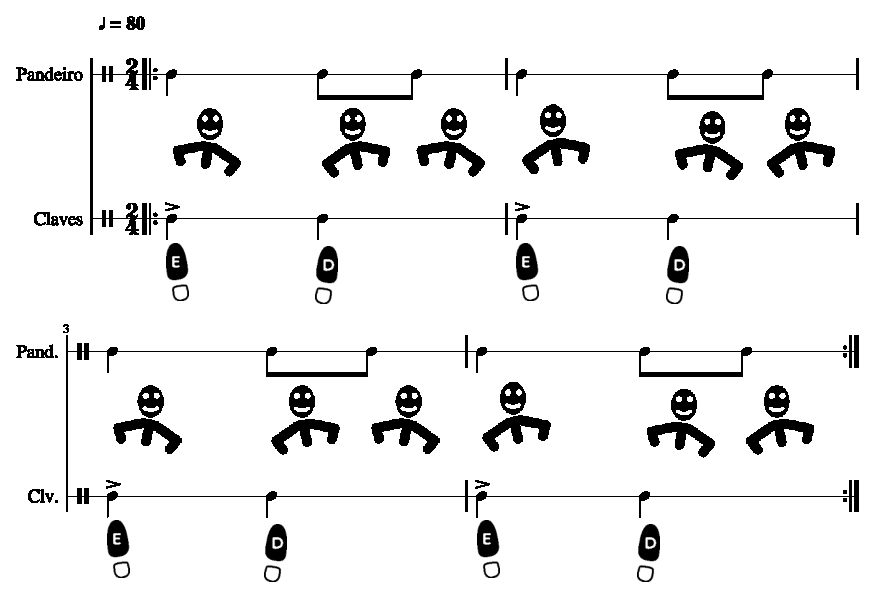
\includegraphics[width=1.0\textwidth]{chapters/cap-body-isolation/bodycontrol1-poliritmia-1.eps}
\caption{Treinando com movimentos policêntricos - ombros e pés.}
\label{fig:bodycontrol1-poliritmia-1}
\end{figure}

Se você já ganhou experiencia com o exercício anterior, 
pode elevar a carga cognitiva agregando alguma atividade a ser realizada em paralelo.

\begin{example}[Agregando atividade externa:]
Podemos evoluir o exercício anterior agregando mais componentes a nosso treinamento cognitivo-motor.
Com este fim podemos agregar o uso de uma bolinha, a qual
jogaremos ao chão e pegaremos ela após o rebote por todo o tempo que dure o treinamento.
Esta componente provocará que nosso cérebro se centre na tarefa de atrapar a bolinha  
e especialize em modo automático o resto de movimentos policêntricos.
\end{example}


\begin{example}[Treinando com movimentos policêntricos - quadril e pés:]
Neste exercício buscaremos desassociar os movimentos do quadril
dos movimentos dos pés.
Para que a desconexão dos movimentos seja treinada a nível cognitivo-motor,
 o quadril e os pés se movimentarão de forma simultânea,
porém seguindo direções diferentes.
\begin{itemize}
\item O quadril terá um movimento circular em sentido anti-horário, com período igual a 2 tempos, 
enquanto que 
\item os pés se movimentarão seguindo um ritmo ``tum tum'', 
\meter{2}{4}\leftrepeat~\Vier\Vier~\rightrepeat, que também tem um período de 2 tempos.
\end{itemize}
Como fonte de informação musical podemos usar qualquer música do samba,
ex: ``Rio antigo'' interpretado por Alcione,
ou alguma melodia simples como a mostrada na Figura \ref{fig:pessoalpesquadril2}.
Na qual temos dois instrumentos musicais que são executados ao mesmo tempo e com o mesmo ritmo,
o pandeiro representa ao movimento do quadril e as claves ao movimento dos pés.
Em todo o exercício o pé esquerdo deve estar ligeiramente adiante do pé direito,
e o peso do corpo deve estar no pé esquerdo quando no movimento circular o quadril passe pela frente,
e o peso do corpo deve estar no pé esquerdo quando o quadril passe por atrás. 
\end{example}

\begin{figure}[!h]
  \centering
    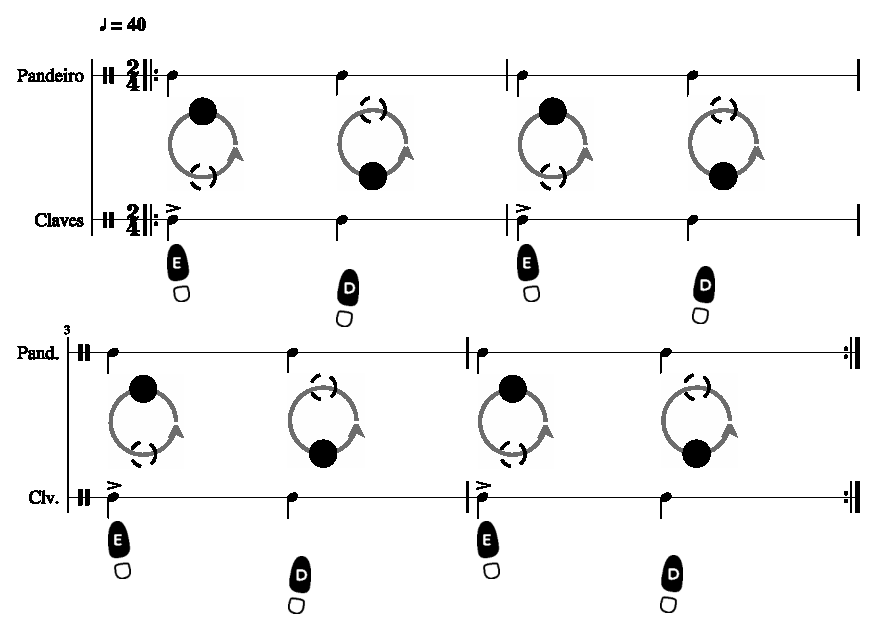
\includegraphics[width=1.0\textwidth]{chapters/cap-body-isolation/bodycontrol2-1.eps}
\caption{Treinando com movimentos policêntricos - quadril e pés.}
\label{fig:pessoalpesquadril2}
\end{figure}

Se o exercício anterior tem sido completamente dominado, podemos treinar deslocar-nos
à direita ou esquerda ou girar sobre nosso próprio eixo, 
enquanto realizamos as trocas de peso.

\begin{example}[Treinando com movimentos policêntricos - quadril e ombros:]
Neste exercício buscaremos desassociar a direção dos movimentos do quadril
dos movimentos dos ombros.
Nosso movimento seguirá um ritmo ``tchic tchic tum'', 
\meter{2}{4}\leftrepeat~\Vier\Acht\Acht~\rightrepeat, 
com uma troca de peso corpo por cada figura musical,
como é mostrado na Figura \ref{fig:pessoalombroquadril1}.
Nesse diagrama cada tempo coreográfico ($TC$)
corresponde a meio tempo musical ($T$), quer dizer $1 TC\equiv  T/2\equiv \Vier/2$,
e $TC3$ e $TC7$ correspondem a tempos fortes do compasso,
nos tempos coreográficos $TC2$ e $TC6$ o peso do corpo está no pé direito em qualquer outro caso estará no pé esquerdo. 
Assim, neste exercício não deslocaremos os pés e
somente realizaremos trocas de peso do corpo, 
tentando em cada troca desassociar a linha do quadril e a dos ombros.

\end{example}

\begin{figure}[!h]
  \centering
  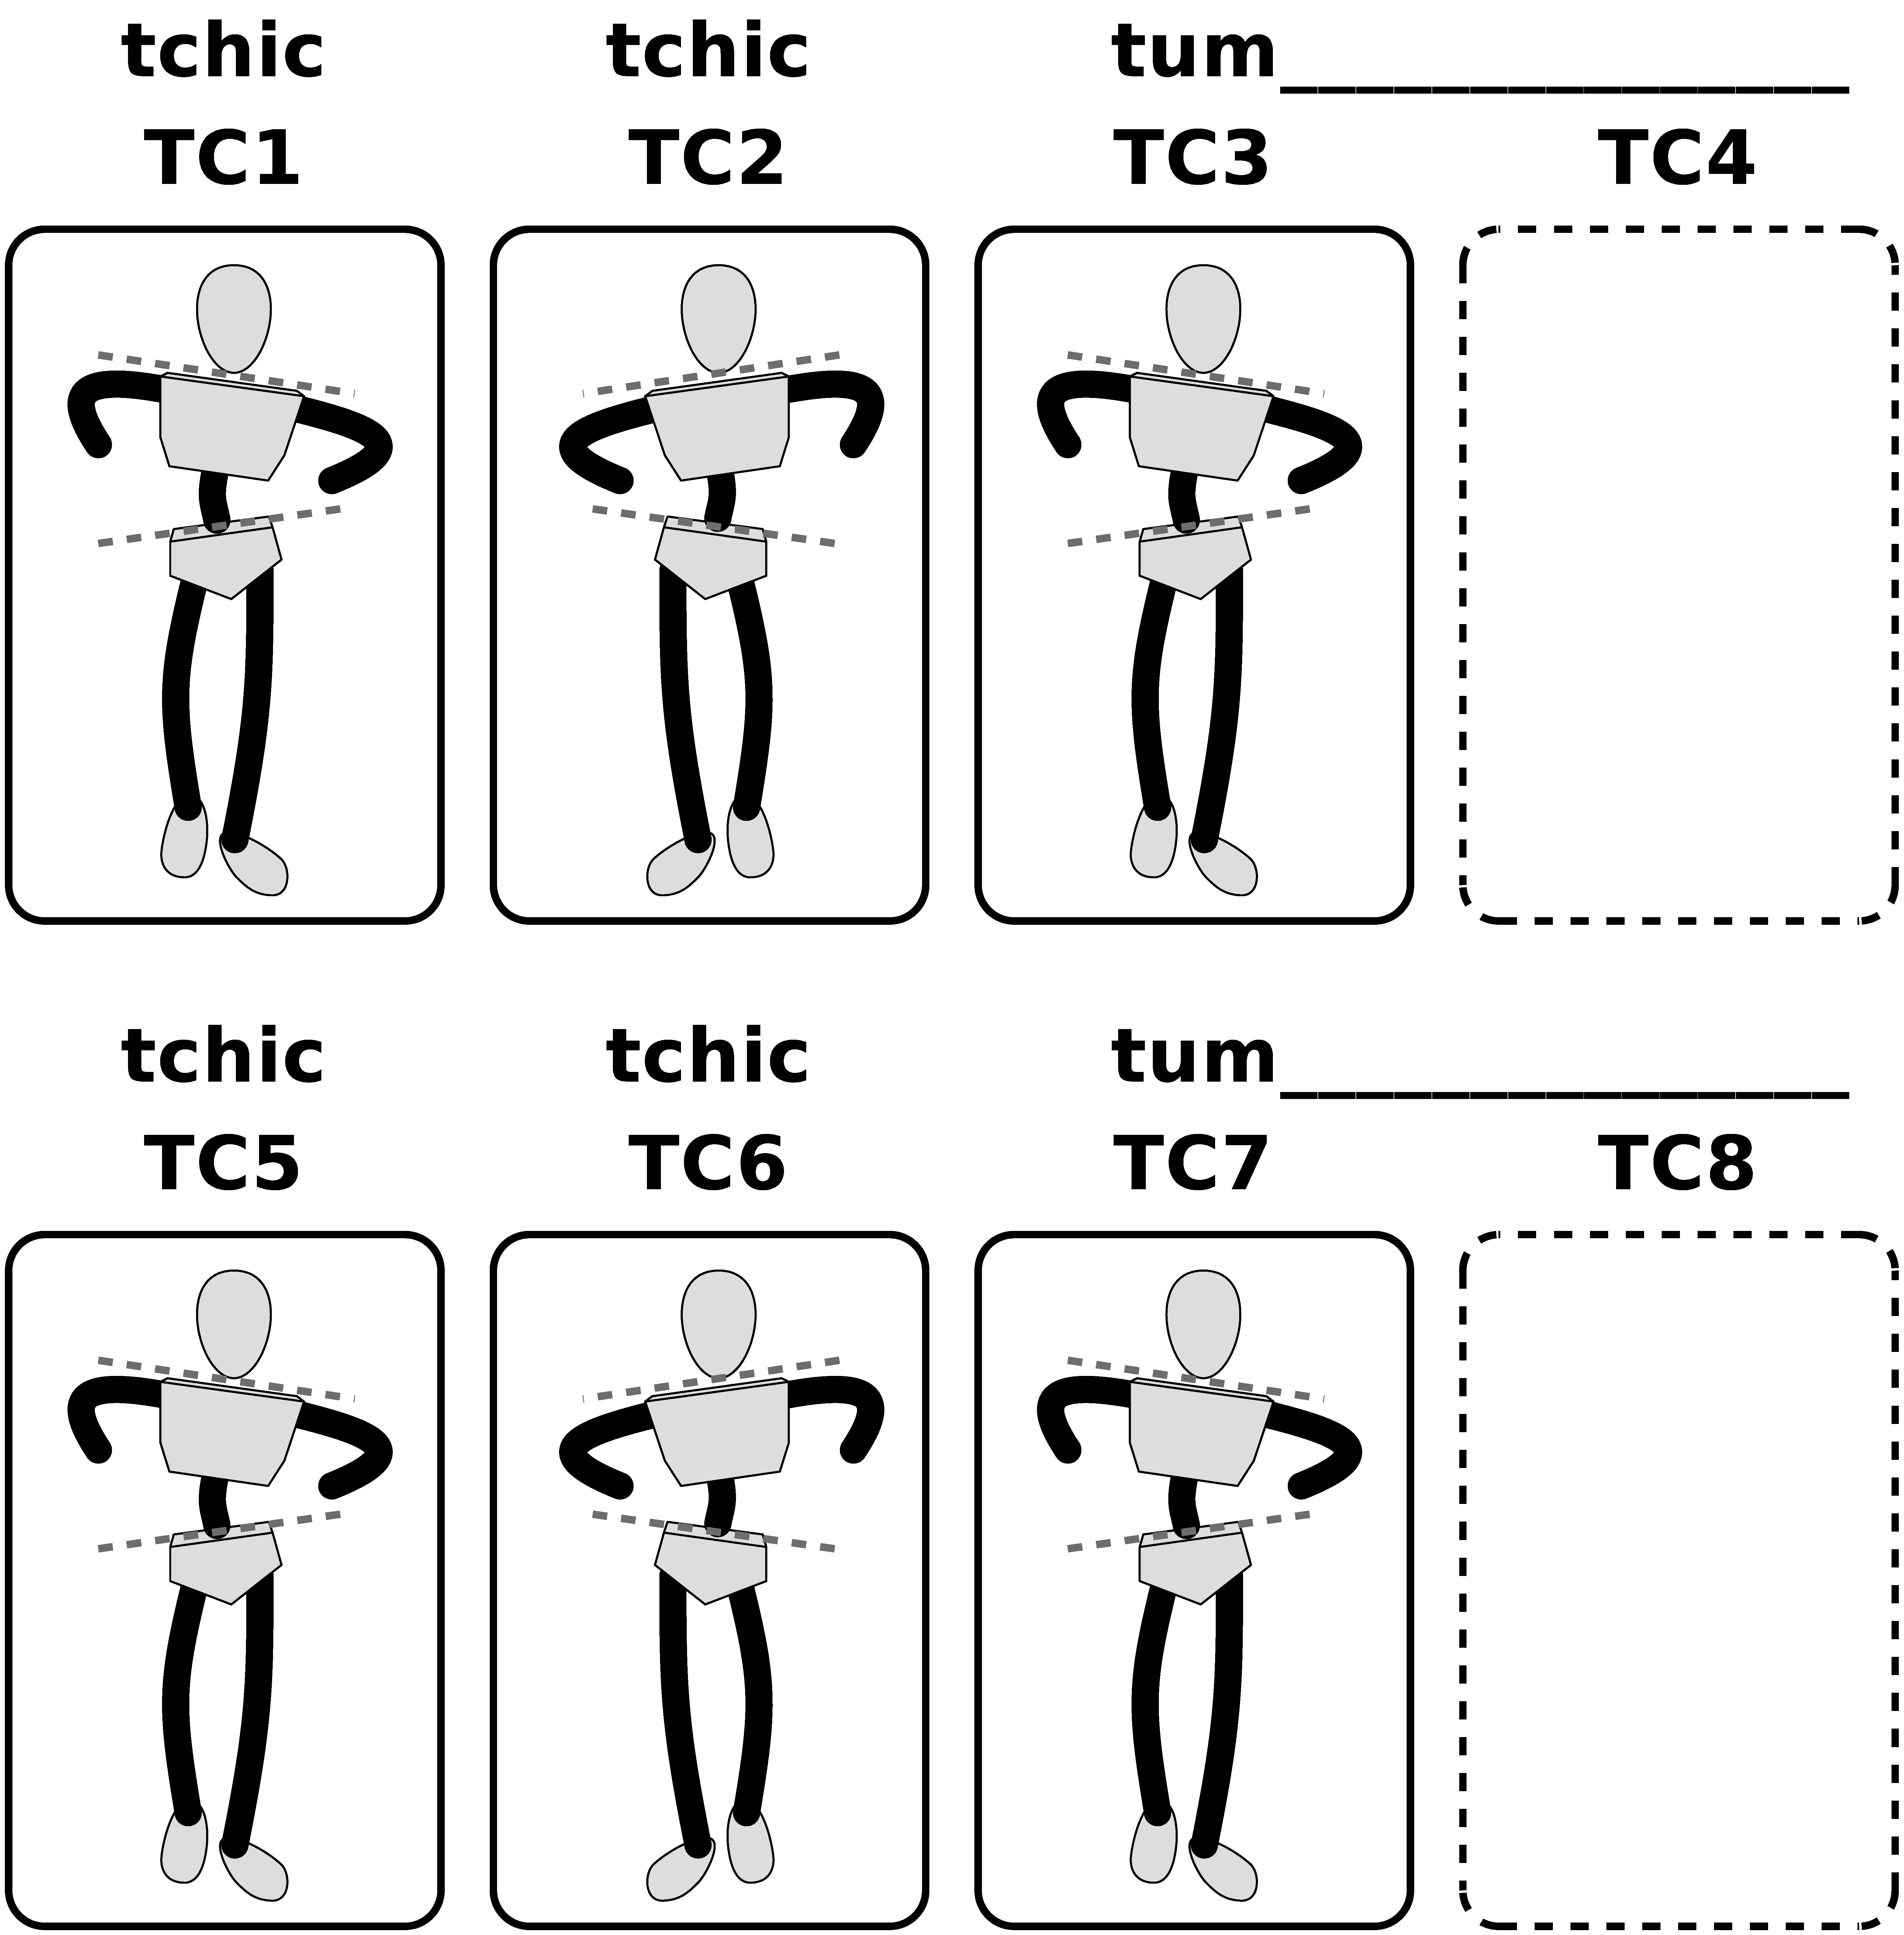
\includegraphics[width=0.65\textwidth]{chapters/cap-body-isolation/postura-ombro2.eps}
\caption{Diagrama de tempos coreográficos para o treino quadril e ombros.}
\label{fig:pessoalombroquadril1}
\end{figure}
